\chapter{Denoising} \label{chap:chap-4}

\section{Introduction}
As the previously discussed dataset was generated using a low-cost potentiostat that lacks the accuracy of commercial options \cite{PabloGarca2024}, we attempt to improve the quality of the data obtained by this potentiostat by applying ML to denoise the raw data with the commercial potentiostat data as a reference.
\section{Autoencoder}
As previously shown in Figure \ref{autoencoder_diagram}, an autoencoder is a neural network used to learn an efficient low-dimensional encoding of data. An autoencoder consists of an encoder and a decoder. The encoder transforms the input data into an encoded representation, and the decoder attempts to recreate the data from the encoded representation. Since the goal is to try and improve the data quality, the commercial potentiostat data is used for the decoder instead. This way, the low-cost potentiostat data is used to create an encoded representation, and an equivalent commercial potentiostat data is decoded. The main problem to solve is how to pair results from the two potentiostats. While the metal and ligand used for each experiment are recorded, numerous other variables can influence the data. Therefore, the challenge revolves around accurately aligning the outcomes generated by the low-cost potentiostat with their counterparts from the commercial one. This alignment is crucial for ensuring the reliability and validity of the encoded representations created by the autoencoder. Without precise pairing, the encoded representations may not accurately capture the underlying patterns in the data, leading to suboptimal performance of the autoencoder. To address this challenge, the clustering technique previously described can be employed. By leveraging the recorded information on metals and ligands, combined with other relevant variables, similar experimental results can be grouped. This clustering process helps in identifying pairs of results that share comparable characteristics, despite potential variations introduced by the different potentiostats.
\section{Results and Discussion}

\begin{figure}[h!]
  \centering
    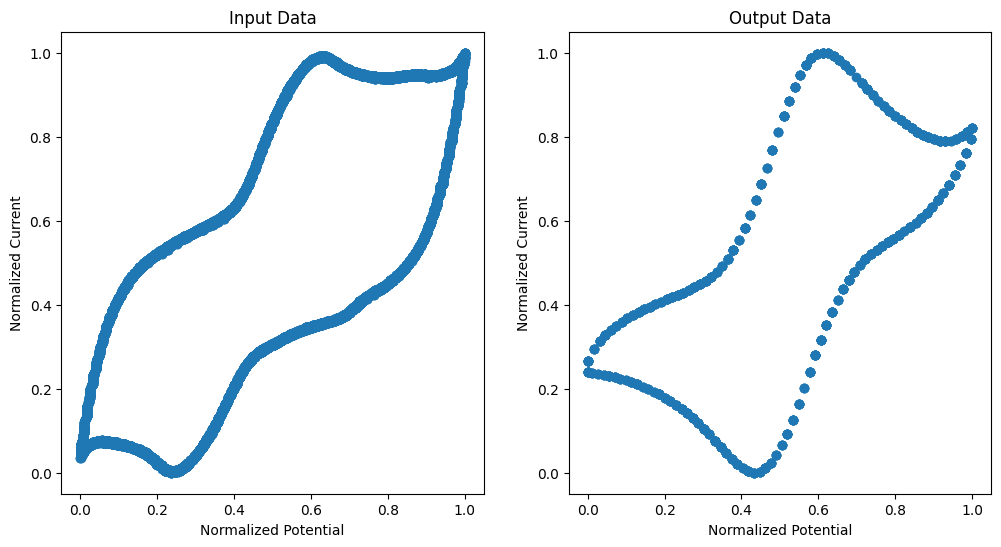
\includegraphics[width=1\textwidth]{figures/autoencoder.png}
    \caption{AutoEncoder Results}
    \label{autoncoder_results}
\end{figure}
In Figure \ref{autoncoder_results}, both the
As seen in Figure \ref{autoncoder_results}, both the input and output are similar in overall shape. However, the output contains a much more defined duck-shaped voltammogram, which is typically expected. The results show promising outcomes and indicate that an autoencoder can effectively transform data from the low-cost potentiostat to resemble data from the commercial potentiostat. By leveraging the capacity of deep neural networks to learn complex patterns and relationships within the data, it becomes feasible to enhance the quality of measurements obtained from low-cost instruments, thereby expanding their utility in research and industrial applications.
However, despite the promising results, several drawbacks and considerations must be acknowledged. Firstly, the effectiveness of the transformation heavily relies on the quality and diversity of the training data. Insufficient or biased training samples may lead to suboptimal performance and generalization issues, especially when dealing with complex electrochemical processes or diverse experimental conditions. While the autoencoder can effectively capture and replicate the dominant features present in the data, it may struggle with preserving subtle nuances or domain-specific characteristics inherent to the commercial potentiostat. Variations in hardware specifics, measurement protocols, or environmental factors could introduce discrepancies between the transformed and reference datasets. 
In conclusion, while autoencoders offer a promising avenue for enhancing the capabilities of low-cost potentiostats, their deployment must be accompanied by rigorous validation and consideration of the aforementioned limitations. Future research could focus on optimizing the autoencoder architecture, exploring alternative deep-learning techniques, and investigating strategies for addressing data heterogeneity to further improve the robustness and versatility of the proposed approach.
